\section{Simulação}
\subsection{Dataset}
\frame{
    \frametitle{Detalhes do dataset}
    \begin{itemize}
    \item Projeto Reality Mining, realizado entre 2004 e 2005 no
    laboratório MIT Media.
    \item 94 usuários monitorados.
    \item Log de informações como:
    \begin{itemize}
        \item Ligações realizadas e recebidas.
        \item ID bluetooth de aparelhos próximos
        \item Identificador da torre associada ao sinal do celular.
    \end{itemize}
    \end{itemize}
} 
\subsection{Redes sociais}
\frame{
    \frametitle{Rede}
    O dataset não fornece uma visão completa da rede.
    \begin{figure}
    \centering
    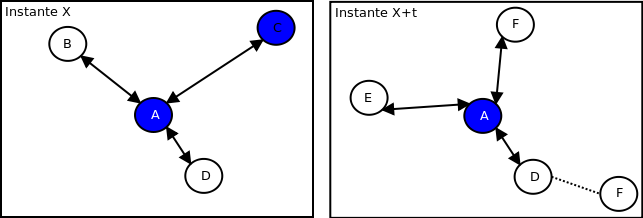
\includegraphics[width=\textwidth]{../doc/img/diagramas/redeSocial.png}
    \caption{Diagrama que ilustra a dinamicidade da rede considerada na
    simulação}
    \label{fig:dinamicidade}
    \end{figure}
}
